\section{Evaluation}
\label{sec:evaluation}

%It is important to keep in mind that although our Syndicate prototype implements a filesystem interface, we did not design Syndicate to be a distributed filesystem.  Our goal is to provide a common interface for organizing data, reading consistent data, and replicating data independently of underlying mechanisms, and a filesystem interface is one of many means to that goal.

Because Syndicate is designed to leverage commodity cloud storage and caching substrates, its absolute performance is bounded by the selected technologies (as well as the workloads). Therefore, to evaluate how well Syndicate performs, we compare it to the performance of these underlying mechanisms. We show that in read-heavy read/write settings, Syndicate lets applications trade good read performance for stronger consistency and good write performance for stronger durability.

\subsection{Testbed}

To test Syndicate, we built a two-tier CDN out of Squid~\cite{Squid} caches, with the top tier running on four VICCI sites~\cite{VICCI} and the bottom tier running on 300 PlanetLab nodes~\cite{PlanetLab}. The VICCI caches were configured to use 1GB of RAM and 8GB of disk using the \texttt{aufs} scheme. The PlanetLab caches were configured to use 256MB of RAM and 1GB of disk space using \texttt{aufs}. To compare Syndicate's consistency scheme with the HTTP RFC cache control scheme~\cite{HTTP-RFC}, we configured our caches to honor server-given object lifetimes, entity tags, and last-modified timestamps, as well as client-given \texttt{If-Modified-Since} and \texttt{If-None-Match} directives.

We deployed the Syndicate MS on Google AppEngine.  Each instance of the MS application ran on a VM with a 600MHz CPU and 128MB of RAM.  We used the High Replication Datastore (HRD) for storing and replicating MS records (where replication is coorinated via Paxos~\cite{paxos}), such that every object record was stored as its own entity group.  We configured the pending request queue to deliver requests to our instances in at most 10 milliseconds (the smallest possible value), and gave the application 10 idling instances.

\subsection{Metadata Operations}

% compare metadata operation time to no-op GET that involves reading something out of ndb
% (can look this up on Google in the worst-case)

Record creations, deletions, and updates run concurrently in the MS if they do not share the same parent, but run sequentially if they do.  To evaluate the performance of the MS on top of Google AppEngine, we had 300 PlanetLab nodes create, read, update, and delete object and directory records.  Each node creates a unique top-level directory named after its hostname (i.e. \texttt{/www.foo.com}), and then an object record (i.e. \texttt{/www.foo.com/obj}).  Each node then reads the metadata along its object's path, updates the object record, and then deletes the object record and directory.

We present the metadata operation times in Figure~\ref{fig:metadata-latency}.  The times are calculated by taking the wall clock time between when the UG began to send data to the MS and when the UG finished receiving a response.  The ``Revalidate'' operation reads the metadata records on the object's path, and is concurrent with all other operations.  The ``Mkdir'' and ``Rmdir'' operations on directories are serialized, since each directory shares the same parent.  The ``Create'', ``Delete'', and ``Update'' operations on objects are concurrent, since each object is in its own directory (and thus has its own parent).

\begin{figure}[h!]
\centerline{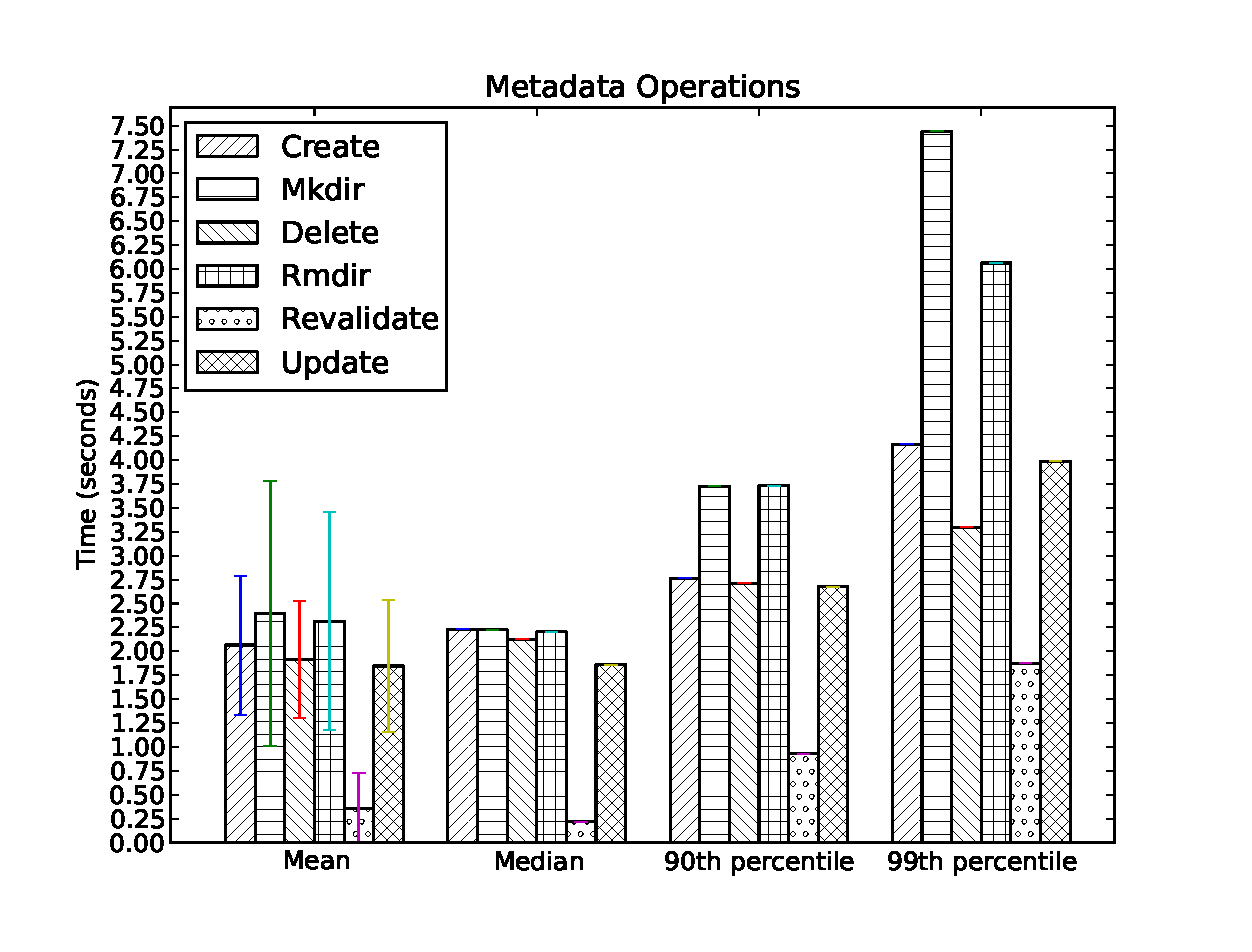
\includegraphics[width=0.55\textwidth]{figures/metadata_operations}}
\label{fig:metadata-latency}
\caption{\it 
Metadata operation latency (in seconds) across 300 PlanetLab nodes.  Error bars are one standard deviation.}
\end{figure}

The latencies with Google AppEngine are surprisingly long, even in the median case.  An initial investigation suggests that they are a combination of RTTs to Google's datacenter and the rather expensive cost of committing a transaction.  Further measurements will reveal the the latency breakdowns of each operation as it executes in the MS.

\subsection{Reads and Consistency}

% local Syndicate read vs local disk read of same number of blocks
% -- compare with/without consistency check
% ----- measure and subtract cost of consistency from Syndicate

% remote Syndicate read (cache miss and hit) vs remote curl read of same blocks on CDN
% -- put Syndicate origin on vcoblitz-cmi
% -- compare with/without consistency check
% ----- measure and subtract cost of consistency from Syndicate

% vary degree of change between writes; measure Syndicate read performance

Reading an object entails periodically checking with the MS to determine if the object has been modified since the last read, and ensuring that the manifest is up-to-date.  To test read performance in the presence of these checks, we had 300 PlanetLab nodes locally read an existing 100-block object, and remotely read a different 100-block object from our CDN a total of 5 times.  The objects both had a $\Delta_{read}$ value of 5 seconds, meaning that remote readers refresh the object's MS record and manifest at the start of each read if they have aged more than 5 seconds.  Each block is 60KB, ensuring that for our read experiments, the object and its manifest can both be completely cached locally.

We measured local object reads and remote object reads separately, since they follow different code paths.  In both cases, we measured the latency of a read as the wall clock time between the start of the read operation and the receipt of the first byte.

For a read on a local object, we measured the latency of reading the local object with and without revalidating its MS record, and compared it to the latency of reading a local file.  The results are presented in Figure~\ref{fig:read_latency_local}.  They show that the latency cost of keeping a local object consistent (relative to simply hosting the data locally and serving it to the CDN) comes almost entirely from the MS, suggesting that local read latency when stronger consistency is desired can be improved simply by picking a faster MS hosting provider.

\begin{figure}[h!]
\centerline{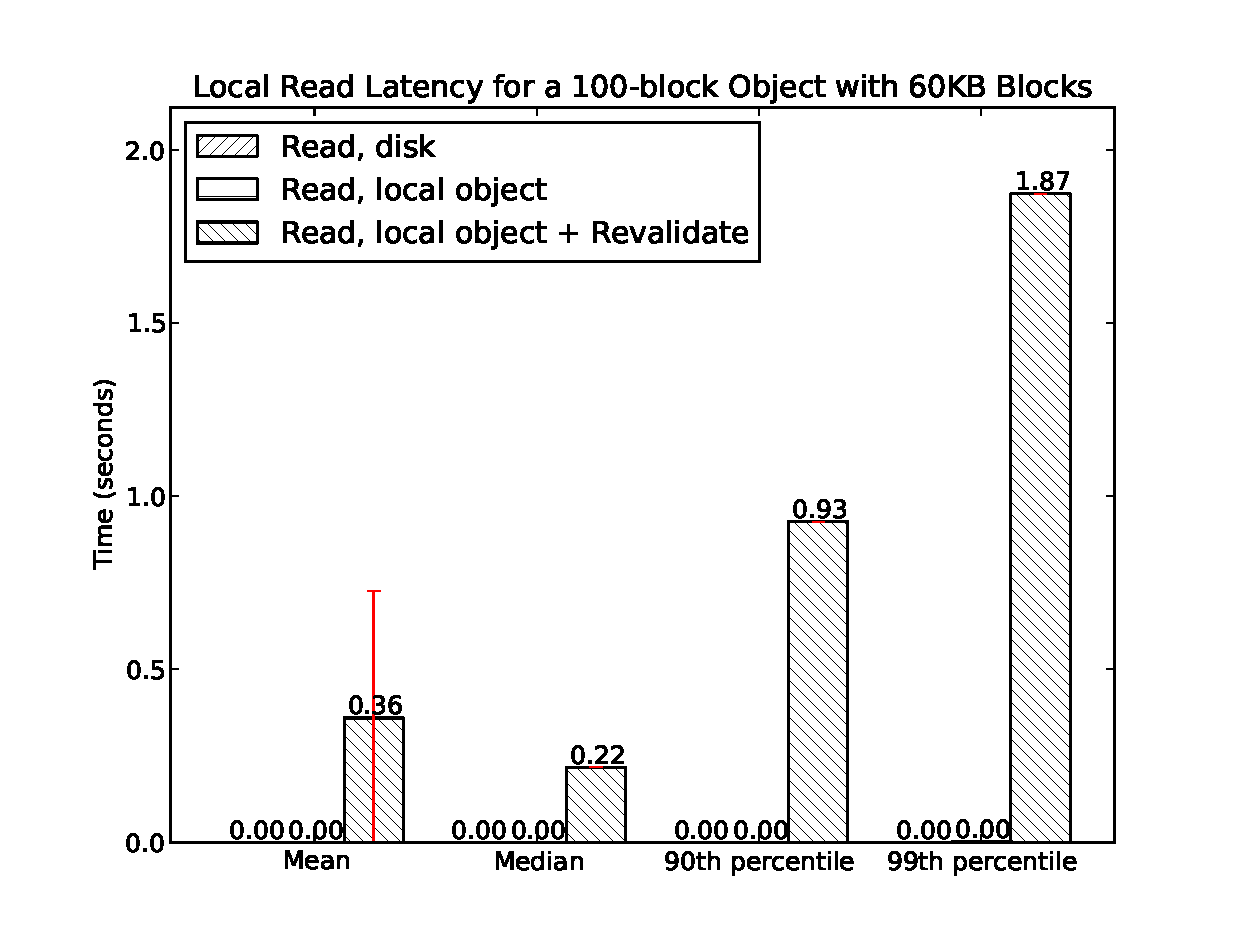
\includegraphics[width=0.55\textwidth]{figures/read_latency_local}}
\label{fig:read_latency_local}
\caption{\it Read latencies on a local object's data.  Error bars are one standard deviation.}
\end{figure}

To measure the read latency on a remote object, we measured the time taken to fetch its manifest from a cold cache, with and without revalidating its record (and in doing so, potentially discovering a new manifest URL).  In order to determine the role of the CDN in adding read latency, we compare these two measurements to the time taken by the \texttt{curl} program to connect to the CDN, request data, and receive the first byte.  The results are presented in Figure~\ref{fig:read_latency_remote}.  They suggest that remote read latency can be reduced by employing lower-latency CDNs (which contribute most of the latency).

\begin{figure}[h!]
\centerline{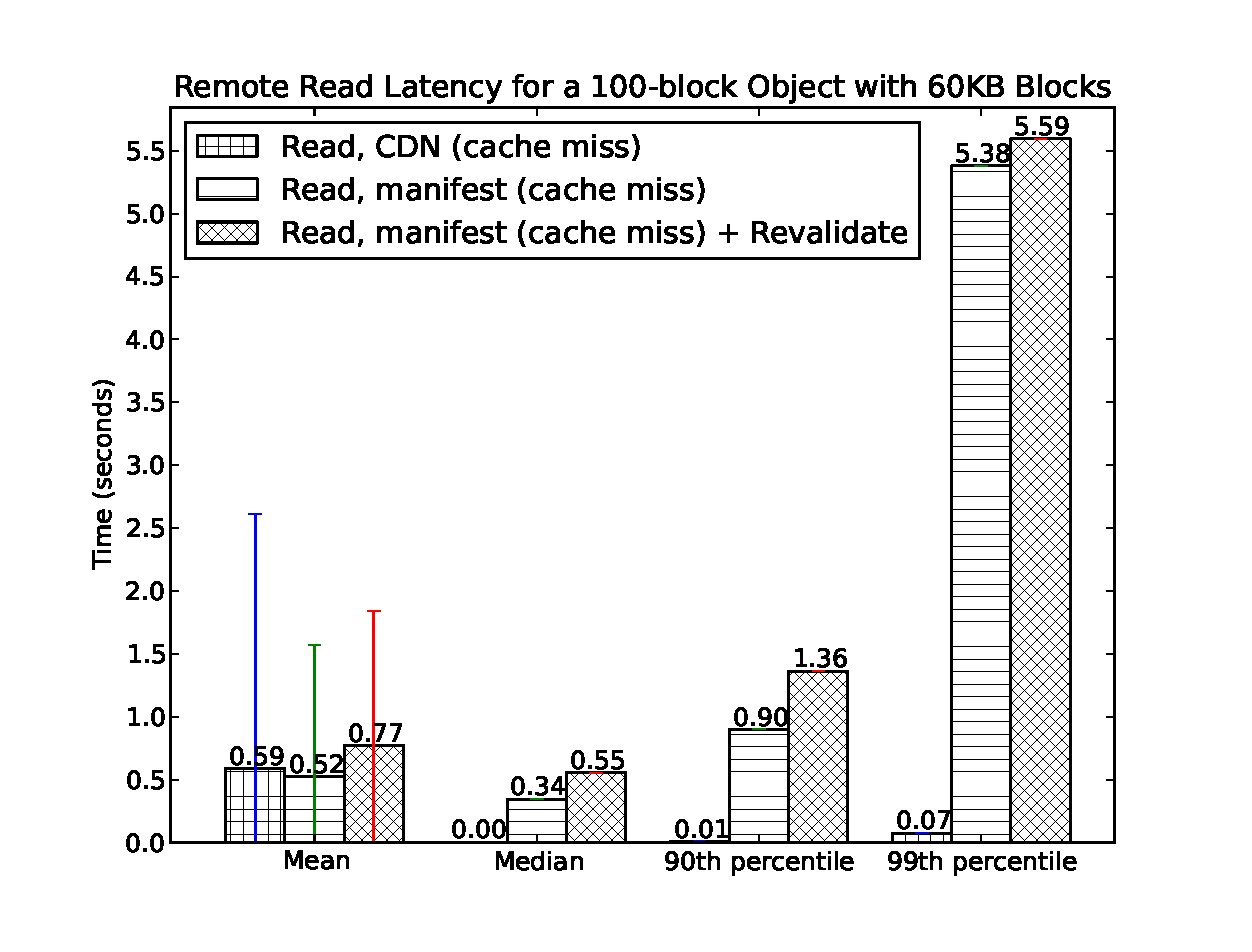
\includegraphics[width=0.55\textwidth]{figures/read_latency_remote}}
\label{fig:read_latency_remote}
\caption{\it Read latencies on a remote object's data.  Error bars are one standard deviation.}
\end{figure}

To understand how Syndicate performs when reading data, we conducted two experiments.  First, we measured the time taken by our UG prototype to read 100 60KB blocks from a locally-hosted object and compared it to directly reading 100 60KB files from local disk.  Second, we measured the time taken by our UG prototype to read 100 60KB blocks from the CDN (with cold and warm caches) and compared it to running \texttt{curl} on each PlanetLab node to read 100 60KB files via the CDN from a common origin server.  We examined only the time taken to read the blocks, not to refresh the manifest and metadata.

The results are presented in Figure~\ref{fig:read_performance}.  They show that a UG's read performance for locally-hosted data is on par with reading the blocks from disk, and that reading block data from the CDN is on par with downloading the same data from the CDN directly.  This suggests that Syndicate's local read performance can be improved by leveraging a faster local disk, and its remote read performance can be improved by leveraging a higher-bandwidth CDN.

\begin{figure*}
\centerline{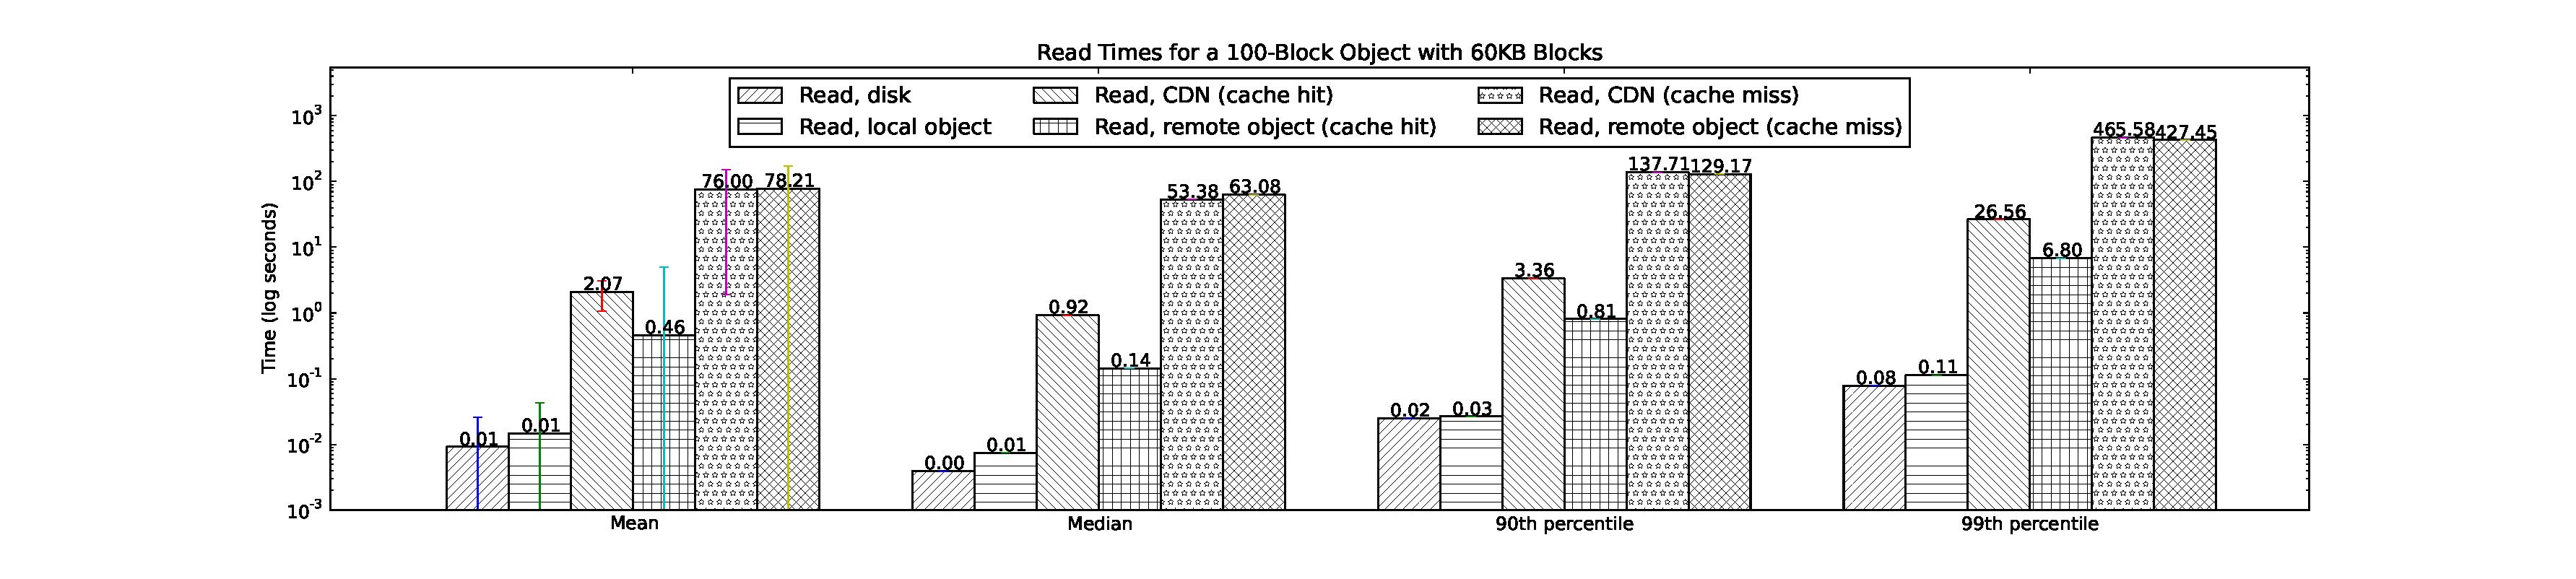
\includegraphics[width=1.2\textwidth]{figures/read_performance}}
\label{fig:read_performance}
\caption{\it
Read performance of Syndicate, as compared against reading blocks directly from disk and directly from the CDN (on both cache hit and miss).  Note that the Y axis is in log-scale.  Error bars are one standard deviation.}
\end{figure*}

The reason Syndicate appears to be faster than \texttt{curl} is because we spawned 100 \texttt{curl} processes to sequentially download the blocks, and piped debugging output from each to disk (but wrote downloaded data to \texttt{/dev/null}).  The time taken to spawn the processes and record debugging output accounts for the difference in performance.  A future experiment could compare Syndicate against a specially-crafted program to fetch the 100 blocks sequentially as a single process.  We expect that it would perform slightly better than Syndicate, since Syndicate must perform some bookkeeping for consistency.

To understand how Syndicate performs when reading remote data after it was written, we hosted a 100-block object on a single UG and had our PlanetLab nodes spawn UGs to read it.  In between reads, we overwrote increasingly large percentages of the object (in 10\% increments) and measured the time taken for the remote UGs to read the block data again.  The times taken to download the object are presented in Figure~\ref{fig:read_after_write}.

\begin{figure}[h!]
\centerline{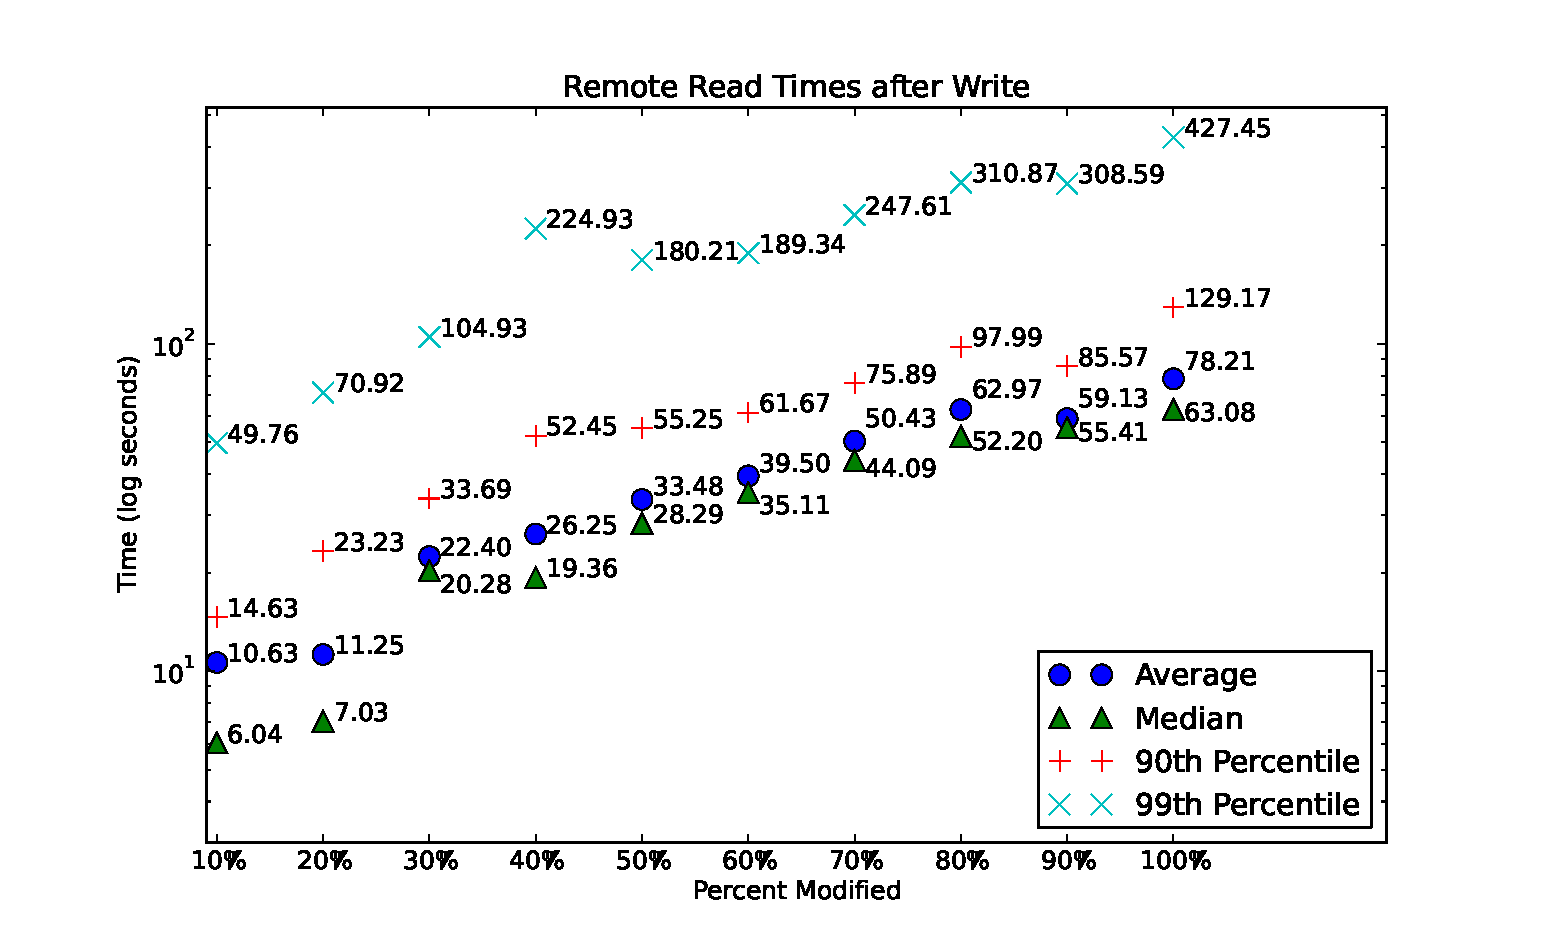
\includegraphics[width=0.55\textwidth]{figures/read_after_write}}
\label{fig:read_after_write}
\caption{\it Times taken to read a remote object after a given percent of its blocks were modified.  Note that the Y axis is in log-scale.}
\end{figure}

The results show that regardless of how fast or slow a UG read data, the time taken to read an object after $X$ blocks are modified increases approximately linearly with $X$.  This is because UGs hit unmodified blocks in the CDN, and only download modified blocks.  Moreover, an initial investigation suggests that the long download times in the 90th and 99th percentiles are due to slow or underprovisioned PlanetLab nodes, not Syndicate.

\subsection{Writes and Durability}

% local write versus Syndicate local write (show where the MS metadata operation comes in)
% remote write versus local write (show where the UG metadata operation comes in)
% -- measure cost of consistency, subtract it out for comparison

Writing to an object entails not only refreshing the object's metadata if it is stale, but also committing new metadata to the MS and replicating data to RGs.  Remote writes additionally entail informing the remote UG that a write has taken place.

To measure the effects of Syndicate's consistency protocol on writes, we had each PlanetLab node create a 100-block object locally.  We measured the time taken to write the blocks to disk, the time taken to propagate the metadata update to the MS, and the time taken to directly write 100 60KB files (revalidating the object's metadata and manifest is the same as for reads, so we did not include them).  The results are presented in Figure~\ref{fig:write_performance}.

\begin{figure}[h!]
\centerline{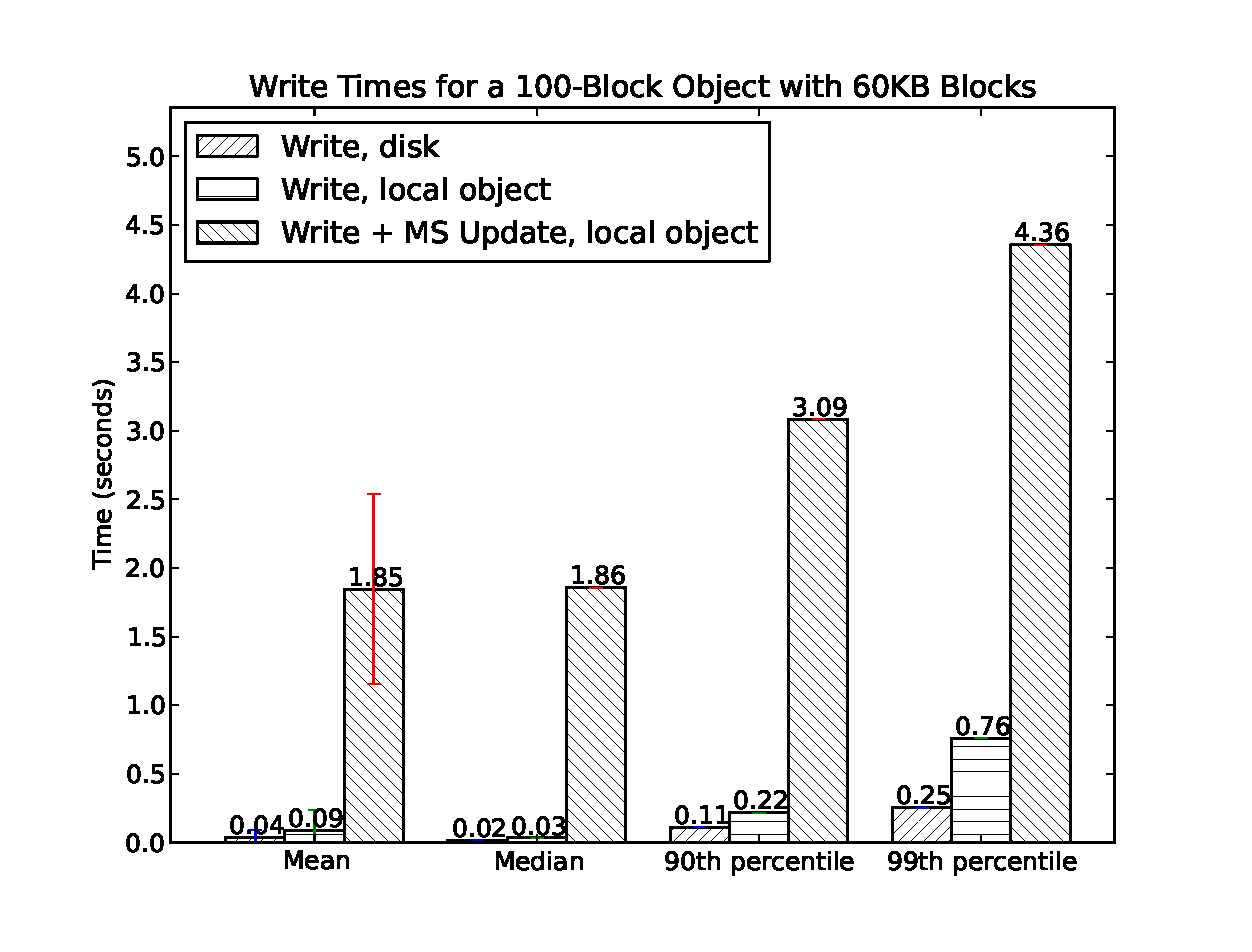
\includegraphics[width=0.55\textwidth]{figures/write_performance}}
\label{fig:write_performance}
\caption{\it Times taken to write a local object's data.  Error bars are one standard deviation.}
\end{figure}.

The results show that without contacting the MS, write performance is between 1.5x to 3x slower with our UG than with writing blocks directly to disk.  However, on further investigation, this penalty is due to the UG's consistency bookkeeping, including updating the object's manifest in RAM and recording new block versions on disk (which entails scanning a directory, unlinking a symlink, and creating a symlink for each block written).

Because of the relatively small object size in this experiment, the time taken to update the object's timestamp on the MS dominates the time taken to perform the write.  As with reads, this latency penalty can be reduced by leveraging a faster MS hosting provider.

\subsection{Future Experiments}

We plan to measure the latency and time consumed by writing a 100-block object in a single UG, and having each PlanetLab node UG overwrite all 100 blocks of the object.  We expect that remote write performance will be similar to the equivalent local write performance, but with the additional RTT of sending the new versions to the remote host.

%To measure the effects of durability, run the above experiments with and without an RG.  We measure the added latency and bandwidth of using an RG to make written data durable.  We compare the latency and bandwith of all eight write configurations (local vs remote, consistency vs no consistency, RG vs no RG) to writing 100 files with the same block size directly (Figure~\ref{fig:writes}).

We also plan to measure the added time required to replicate data on write.  We would measure the latency of propagating data to an RG, as well as the time taken by the RG to begin replicating data to the underlying store.  We would compare the time needed to replicate the data via the RG to the time needed to replicate the data manually.

We additionally plan to measure the time taken for a UG to become the acting owner of an object if the remote object cannot be read or written.  We would measure the time taken by the UG to detect the failed owner, the time taken by the MS to process the change, and the time taken for the remaining UGs to detect the change in ownership.  We would additionally measure the effect of an ownership change on read and write aggregate bandwidth from the remaining UGs.

\subsection{Discussion}

The effect of Syndicate's architecture is that the performance of the system is predictable by its underlying storage and caching mechanisms, the desired level of consistency, and the desired level of durability.  The performance of a metadata operation can be determined by the latency and bandwidth of the cloud-computing platform that hosts the metadata, as well as the amount of contention on a single parent record.  Users can achieve maximal metadata concurrency with Syndicate by ensuring that object records do not share a parent.  Moreover, users can improve Syndicate's metadata performance by choosing a faster underlying store.

The performance of a read operation is determined by how long the RTT is to the MS, how often the object is checked for freshness, and how quickly either underlying storage (for locally-hosted objects) or caching infrastructure (for remote objects) can deliver data.  Users can improve Syndicate's read performance by choosing less consistency, a faster MS, faster underlying storage, and/or a more scalable CDN.

Similarly, the performance of a write operation on an object is determined by the RTT to the MS, the bandwidth of underlying storage, the RTT to the UG, and the latency and bandwidth of sending data to the RG.  The user can configure write performance by changing the consistency and durability requirements, choosing better underlying infrastructure, and varying the number of RGs in the Volume.

